\documentclass[a4paper]{article}
\usepackage[utf8]{vietnam}
\usepackage{scrextend}
\changefontsizes{13pt}
\usepackage{xcolor}
\usepackage{titlesec}
\usepackage{mdframed}
\usepackage{amsmath}
\usepackage{array}
\usepackage[amsmath,standard,thmmarks]{ntheorem}
\usepackage{amssymb}
\usepackage{exscale}
\usepackage{amsfonts}
\usepackage{eucal}
\usepackage{enumerate}
\usepackage{enumitem}
\usepackage{commath}
\usepackage[dvips]{color}
\usepackage{graphicx}
\usepackage{tcolorbox}
\usepackage{url}
\usepackage[unicode]{hyperref}
\newmdenv[linecolor=black,skipabove=\topsep,skipbelow=\topsep,
leftmargin=-5pt,rightmargin=-5pt,
innerleftmargin=5pt,innerrightmargin=5pt]{mybox}
\setlength{\parindent}{0pt}
 \usepackage[left=2cm,right=2cm,top=2.5cm,bottom=2.5cm]{geometry}
\renewcommand{\baselinestretch}{1.5}
\newcommand{\heva}[1]{\left\{ 
\begin{aligned}#1\end{aligned}\right.}

\theoremstyle{nonumberplain} 
\theoremheaderfont{\itseries\slshape} 
\theorembodyfont{\normalfont}
\theoremsymbol{\ensuremath{_\blacksquare}} 
\renewtheorem{proof}{Chứng minh:}
\newcommand{\chm}[1]{\begin{proof}#1\end{proof}}

\usepackage{fancyhdr}
\pagestyle{fancy}
\fancyhf{}
\lhead{BTL1 - Mô hình hóa thống kê}
\cfoot{\thepage}
\rhead{Nhóm 4}
\title{BÀI TẬP LẦN 1 - MHHTK}

\author{NHÓM 4}

\date{\today}%

\begin{document}

\begin{titlepage}
\thispagestyle{empty}
\begin{center}
\textbf{\large{TRƯỜNG ĐẠI HỌC KHOA HỌC TỰ NHIÊN TP.HCM}\\
CAO HỌC KHÓA 30}\\
---------------*---------------
\end{center}
\vspace{0.3cm}
\begin{center}

\includegraphics[scale=0.8]{Logo-Math-CS.png} 
\end{center}
\vspace{0.7cm}
\begin{center}
\textbf{\Large{\textcolor[rgb]{1.0,0.0,0.0}{Bài tập lần 1}}}\\
\vspace{0.5cm}
\textbf{\Large{\textcolor[rgb]{1.0,0.0,0.0}{MÔ HÌNH HÓA THỐNG KÊ}}}\\
\vspace*{4cm}
$\begin{array}{rl}
\text{\large{Giảng viên hướng dẫn:}} &\text{\large{\bf TS. Nguyễn Thị Mộng Ngọc}}  \\
\vspace*{1cm}
\text{\large{Nhóm thực hiện:}}     & \text{\large{\textbf{Nhóm 4}}}
\end{array}$\\
\vspace{4cm}
\normalsize{TP. Hồ Chí Minh $-$ Tháng 01, 2021}
\end{center}
\end{titlepage}

\newpage
\thispagestyle{empty}
\begin{center}
\textbf{\large{BẢNG PHÂN CÔNG CÔNG VIỆC}\\}
\vspace{1cm}
\begin{tabular}{|m{4.5cm}||m{8cm}|m{3.5cm}|} 
\hline
\textbf{Thành viên} & \centering{\textbf{Công việc}} & \textbf{Mã số học viên}\\
\hline
1. Đặng Khánh Thi & $-$ Code R bài 1& \\
& $-$ Kiểm tra code R bài 2, bài 3 & 20C29038 \\
& $-$ Thảo luận ghi nhận xét 3 bài & \\
\hline
2. Đinh Thị Nữ  & $-$ Code R bài 2& \\
& $-$ Kiểm tra code R bài 1, bài 3& 20C29013\\
& $-$ Thảo luận ghi nhận xét 3 bài& \\
\hline 
3. Lý Phi Long & $-$ Code R bài 3& \\
& $-$ Kiểm tra code R bài 1, bài 2& 20C29028\\
& $-$ Thảo luận ghi nhận xét 3 bài& \\
\hline
4. Phan Thị Thùy An & $-$ Tổng hợp, kiểm tra code R bài 1,2,3 & \\
Nhóm trưởng & $-$ Thảo luận ghi nhận xét 3 bài & 20C29002 \\
& $-$ Trình bày file nhận xét bằng Latex & \\
\hline
\end{tabular}
\end{center}

\newpage
\section*{Exercise 1 (2.8.1 page 38)}
$Y = \beta_0 + \beta_1 x + e$ where $Y$ is the gross box
office results for the current week (in \$) and $x$ is the gross box office results for the
previous week (in \$).\\
\textbf{(a) Find a 95\% confidence interval for the slope of the regression model, $\beta_1$. Is 1 a plausible value for $\beta_1$?}
\begin{center}
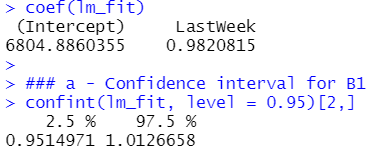
\includegraphics[scale = 0.8]{1a.PNG} 
\end{center}
Dựa vào kết quả mô hình, ta tìm được 95\% khoảng tin cậy cho giá trị $\beta_1$ là  $[0.9515 ; 1.0127]$

Nhận thấy giá trị 1 thuộc khoảng tin cậy của $\beta_1$, vì vậy có thể xem $\beta_1 = 1$.

\textbf{(b) Test the null hypothesis $H_0: \beta_0 = 10000$ against a two-sided alternative.}
\begin{center}
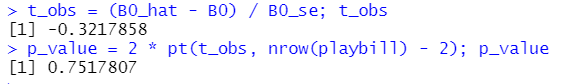
\includegraphics[scale = 0.8]{1b.PNG} 
\end{center}
Với $p_{value} = 0.75 \nless \alpha_{default}=0.05 $ chúng ta không đủ cơ sở để bác bỏ giả thuyết $H_0$.

\textbf{(c) Find a 95\% prediction interval for the gross box office results for the current week (in \$) for a production with \$400,000 in gross
box office the previous week. Is \$450,000 a feasible value for the gross box
office results in the current week, for a production with \$400,000 in gross
box office the previous week? }
\begin{center}
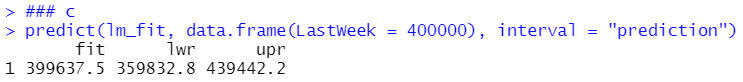
\includegraphics[scale = 0.8]{1c.PNG} 
\end{center}
Dễ nhận thấy $450000$ không thuộc khoảng dự đoán $[359832.8; 439442.2]$ của mô hình, nên nó không là giá trị phù hợp.

\textbf{(d) Some promoters of Broadway plays use the prediction rule that next week’s gross box office results will be equal to this week’s gross box office results.}
\begin{center}
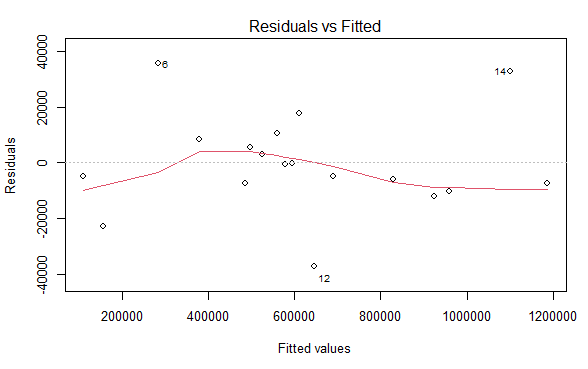
\includegraphics[scale = 0.8]{1d.PNG} 
\end{center}
Dựa vào biểu đồ Residuals vs Fitted, ta thấy rằng chiến thuật dự đoán doanh số tuần hiện tại so với tuần trước là một chiến lược khá hợp lý. \\
Tuy nhiên, có ít nhất 3 điểm bị lệch khỏi đường hồi quy.\\
Vì vậy, họ cần thêm dữ liệu để có cái nhìn khách quan hơn hoặc dùng một mô hình khác có thể tạo ra quy tắc dự đoán tốt hơn, giảm thiểu rủi ro.

\section*{Exercise 2 (2.8.2 page 38)}
$Y = \beta_0 + \beta_1 x + e$ where 
$Y$ = Percentage change in average price from July 2006 to July 2007; and $x$ = Percentage of mortgage loans 30 days or more overdue in latest quarter.

\textbf{(a) Find a 95\% confidence interval for the slope of the regression model, $\beta_1$. On the basis of this confidence interval decide whether there is evidence of a significant negative linear association.}
\begin{center}
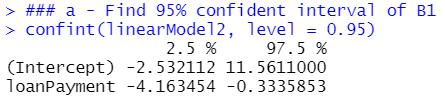
\includegraphics[scale = 0.8]{2a.PNG} 
\end{center}
Dựa vào kết quả mô hình, ta tìm được 95\% khoảng tin cậy cho giá trị $\beta_1$ là   $[-4.16;-0.33]$.

Ta có dạng tổng quát của mô hình hồi quy tuyến tính được cho là: $$Y = 4.514 - 2.249x$$ nên $Y$ và $x$ có mối tương quan nghịch hay $x$ tăng thì $Y$ giảm và ngược lại.

\textbf{(b) Use the fitted regression model to estimate $E(Y |X=4)$. Find a 95\% confidence interval for $E(Y |X=4)$. Is 0\% a feasible value for $E (Y |X=4)$?}

\begin{center}

\includegraphics[scale = 0.8]{2b.PNG} 
\end{center}

Dựa vào mô hình tổng quát mối liên hệ giữa 2 biến $x$ và $Y$ ta tính được giá trị ước lượng của $Y$ tại $ x = 4$   là $Y = -4.48$\\
Tương tự ta tính được 95\% độ tin cậy của $Y$ khi  $x = 4$ nằm trong khoảng $[-6.6;-2.3] $\\
Vì 95\% độ tin cậy của y khi $x = 4$ nằm trong khoảng  $[-6.6;-2.3]$ nên 0\% không phải là giá trị mong đợi phù hợp khi $x = 4$.

\section*{Exercise 3 (2.8.3 page 38)}
$Y = \beta_0 + \beta_1 x + e$ where 
$Y$ is the processing time and $x$ is the
number of invoices.

\textbf{(a) Find a 95\% confidence interval for the start-up time, i.e., $\beta_0$.}

\begin{center}
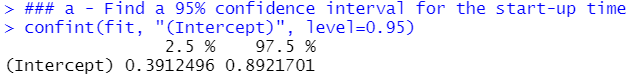
\includegraphics[scale = 0.8]{3a.PNG} 
\end{center}

Dựa vào kết quả mô hình, ta tìm được 95\% khoảng tin cậy cho giá trị $\beta_0$ là $[0.3912;0.8922]$

\textbf{(b) Test the null hypothesis
$H_0: \beta_1 = 0.01$ against a two-sided alternative.}

\begin{center}

\includegraphics[scale = 0.8]{3b.PNG} 
\end{center}
$\beta_1 = 0.01$ nằm trong khoảng tin cậy vừa tìm được, do đó chưa đủ cơ sở để bác bỏ $H_0$ với mức ý nghĩa $\alpha = 5\%$ 

\textbf{(c) Find a point estimate and a 95\% prediction interval for the time taken to process 130 invoices.}

\begin{center}
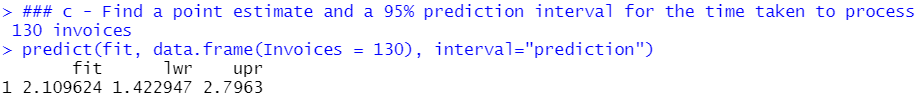
\includegraphics[scale = 0.8]{3c.PNG} 
\end{center}
Dựa vào mô hình dự đoán, thời gian cần để xử lý 130 hóa đơn là 2.1 giờ với khoảng tin cậy 95\% là $[1.4; 2.8]$ hours.
\end{document}
